\section{Aproksymacja średniokwadratowa}
%%%%%%%%%%%%%%%%%%%
\begin{frame}{Aproksymacja średniokwadratowa}
  	\begin{figure}
	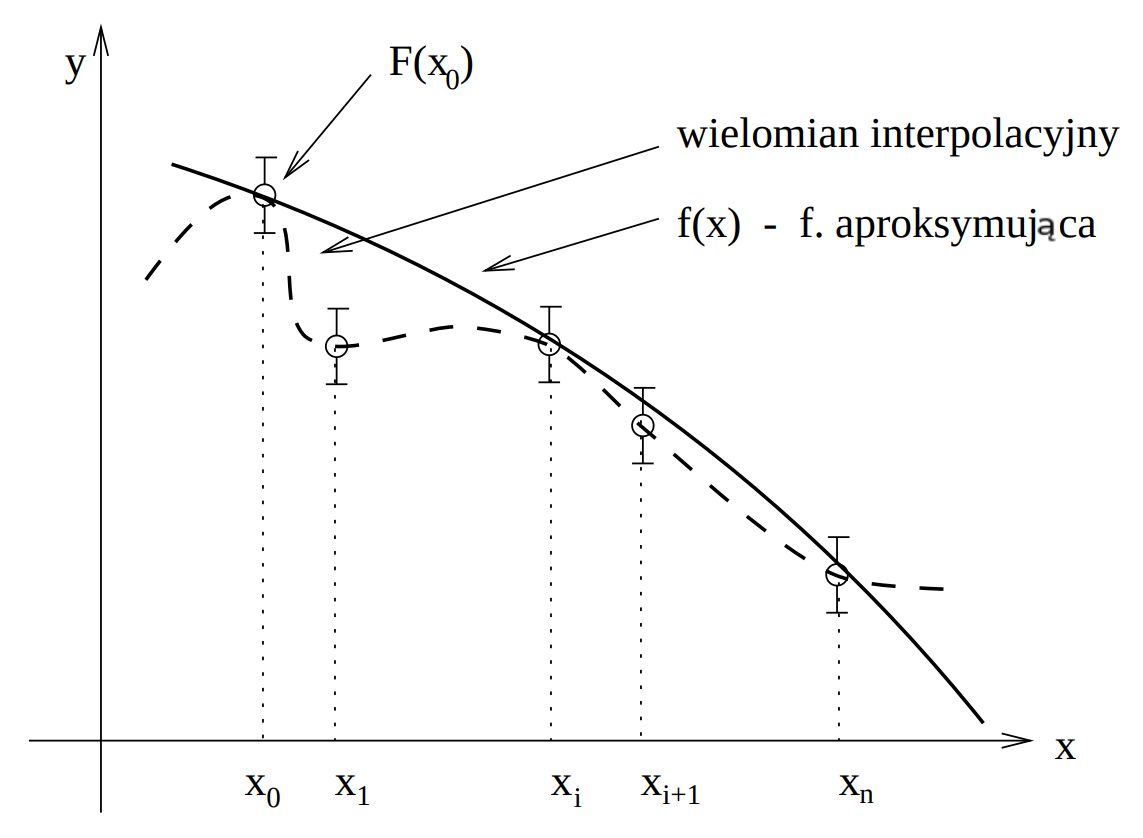
\includegraphics[height=0.8\textheight]{img/5/aproksymacja_sredniokwadratowa}
	\end{figure}
\end{frame}
%%%%%%%%%%%%%%%%%%%
\begin{frame}{Postawienie problemu}
	\textbf{Dane:}\newline
    - ${(x_i,y_i = F(x_i)),i=0,1,\ldots,n}$, czyli mamy (n+1) węzłów \newline
    - układ funkcji bazowych: $\varphi_j(x), j=0,1,\ldots,m$.\newline\par
    \textbf{Szukamy wielomianu uogólnionego:}
    $$f(x) = \sum_{j = 0}^{m} a_j \varphi_j(x)$$
    czyli $\{{a_j}\}_{j=0}^m$, dla których:
    $$min!\parallel F(x) - f(x) \parallel = min!\underbrace{ \sum_{i=0}^{n}w(x_i)\underbrace{\bigg[F(x_i)-\sum_{j=0}^{m}a_j\varphi_j(x_i)\bigg]^2}_\text{odchylenie}}_{H(a_0,a_1,\ldots,a_m)}$$
    \textbf{Pochodzenie nazwy:} postać normy $F(x)$ na $[a,b]$
\end{frame}
%%%%%%%%%%%%%%%%%%%
\begin{frame}{Przypadek ciągły}
    Dla przypadku ciągłego minimalizujemy wartość całki:
    $$min!\int_a^bw(x)[F(x)-f(x)]^2dx% : \sum \rightarrow \int
    $$
    $\Rightarrow$ aproksymacja średniokwadratowa funkcji ciągłych\newline

    $w(x)$ - funkcja wagowa, $w(x)\geqslant0$ ((jak dla iloczynu skalarnego))\newline
    Zwykle: $w(x_i) \sim \frac{1}{[\text{błąd }F(x_i)]^2}$ lub $w(x) = 1$
\end{frame}
\begin{frame}{Współczynniki wielomianu uogólnionego}
    Współczynniki $\{a_j\}$ znajdujemy z warunku: $\frac{\partial H}{\partial a_k} = 0, k=0,1,\ldots,m$
    $\Rightarrow$ układ $(m+1)$ równań liniowych o $(m+1)$ niewiadomych
    $$\frac{\partial H}{\partial a_k} = -2 \cdot \sum_{i=0}^{n}w(x_i)\bigg[F(x_i)-\sum_{j=0}^{m}a_j\varphi_j(x_i)\bigg]\varphi_k(x_i)=0;k=0,1,\ldots,m$$
    Jest to \textbf{układ normalny.}
\end{frame}
%%%%%%%%%%%%%%%%%%%
\begin{frame}{Aproksymacja wielomianowa}
	funkcje bazowe $\rightarrow$ ciąg jednomianów $\varphi_j(x) = x^j,j=0,1,\ldots,m$\newline
    funkcje aproksymująca: $f(x) = \sum_{j=0}^{m}a_j\varphi_j(x)=\sum_{j=0}^{m}a_jx^j$ \newline
    $F(x)$ - na zbiorze dyskretnym $\{x_i\},i=0,1,\ldots,n$
    $$min!\sum_{i=0}^{n}w(x_i)[F(x_i)-f(x_i)]^2 \rightarrow$$
    układ normalny:
    $$\sum_{i=0}^{n}w(x_i)\bigg[F(x_i)-\sum_{j=0}^{m}a_jx_i^j\bigg]x_i^{k\leftarrow\frac{\partial f}{\partial a_k}}=0,k=0,1,\ldots,m$$
    $$\sum_{i=0}^{n}w(x_i)x_i^k\sum_{j=0}^{m}a_jx_i^j=\sum_{i=0}^{n}w(x_i)F(x_i)x_i^k,k=0,1,\ldots,m$$
    $$\sum_{j=0}^{m}\underbrace{\bigg(\sum_{i=0}^{n}w(x_i)x_i^{j+k}\bigg)}_{g_{k,j}}a_j = \underbrace{\sum_{i=0}^{n}w(x_i)F(x_i)x_i^k}_{b_k}$$
\end{frame}
%%%%%%%%%%%%%%%%%%%
\begin{frame}
	W postaci macierzowej:
    \begin{center}
    	 $\left(\begin{array}{ccccc}
    \sum w_i & \sum w_ix_i & \sum w_ix_i^2 & \ldots & \sum w_i x_i^m \\
    \sum w_ix_i & \sum w_ix_i^2 & \sum w_ix_i^3 & \ldots & \sum w_i x_i^{m+1} \\
    . & . & . & . & . \\
    \sum w_ix_i^m & \sum w_ix_i^{m+1} & \sum w_ix_i^{m+2} & \ldots & \sum w_i x_i^{2m}
    \end{array}\right)
    \left(\begin{array}{c}
    	a_0 \\ a_1 \\ \vdots \\ a_m
    \end{array}\right) =\newline=
    \left(\begin{array}{c}
    	\sum w_iF_i\\
        \sum w_i F_i x_i \\
        \vdots \\
        \sum w_i F_i x_i^m
    \end{array}\right)$
    \end{center}
    \begin{center}
    	\underline{$G \cdot A = B$}
    \end{center}
   	
\end{frame}
%%%%%%%%%%%%%%%%%%%
\begin{frame}
	\textbf{Jeżeli:}
    \begin{enumerate}
    \item $x_0,x_1,\ldots,x_n$ - są różne
    \item $m \leqslant n$
    \end{enumerate}
    to $det G \not= 0 \rightarrow$ układ ma jedno rozwiązanie. 
    \begin{flushright}
    	\textit{Zadanie: } \quad Pokazać, że dla $m = n$ - wiel. aproksymacyjny = interpolacyjny $(H=0)$
     \end{flushright}
\end{frame}
%%%%%%%%%%%%%%%%%%%
\begin{frame}{W praktyce}
	\begin{itemize}
	\item $m \ll n$ (korzystamy z dużej ilości informacji)
    \item $m$ - wysoki - by dobrze przybliżyć funkcję
    \item $m$ - niski - by wygładzić błędy
    \item zwykle $m \leqslant 6$
	\end{itemize}
\end{frame}
%%%%%%%%%%%%%%%%%%%
\begin{frame}{Ortogonalność funkcji}
	\begin{block}{Definicja ortogonalności funkcji}
	Funkcje $f(x)$ i $g(x)$ nazywamy ortogonalnymi na dyskretnym zbiorze punktów $\{x_i,i=0,1,..,n\}$, jeżeli:
    $$\sum_{i=0}^{n}f(x_i)\cdot g(x_i) = 0, \sum_{i=0}^{n}[f(x_i)]^2 > 0,\sum_{i=0}^{n}[g(x_i)]^2 > 0$$
	\end{block}
\end{frame}
%%%%%%%%%%%%%%%%%%%
\begin{frame}{Ortogonalność ciągów}
	\begin{block}{Definicja ortogonalności ciągów}
	Ciągi funkcyjne $\{\varphi_k(x)\}$ nazywamy ortogonalnymi na dyskretnym zbiorze punktów $\{x_i\}$, jeżeli:
    $$\sum_{i=0}^{n}\varphi_j(x_i)\varphi_k(x_i) = \left\{\begin{array}{cl}
    	0 & j \not= k \\
        >0 & j = k \quad \rightarrow (*)
    \end{array}\right.$$
    $(*)$ - nie wszystkie $x_i$ to miejsca zerowe.
	\end{block}
\end{frame}
%%%%%%%%%%%%%%%%%%%
\begin{frame}{Aproksymacja średniokwadratowa wielomianami ortogonalnymi}
	Dla wielomianów ortogonalnych układ normalny:
    $$\sum_{i=0}^{n}w(x_i)\Bigg[F(x_i)-\underbrace{\sum_{j=0}^{m}a_j\varphi_j(x_i)}\Bigg]\varphi_k(x_i)=0, k=0,1,..,m$$
    \begin{center}
    	$$\sum_{i=0}^{n}w(x_i)F(x_i)\varphi_k(x_i)=\sum_{i=0}^{n}w(x_i)\varphi_k(x_i)\sum_{j=0}^{m}a_j\varphi_j(x_i)=$$\newline
        $$=\sum_{j=0}^{m}a_j\sum_{i=0}^{n}w(x_i)\varphi_k(x_i)\varphi_j(x_i) = a_k\sum_{i=0}^{n}w(x_i)\varphi_k^2(x_i)$$
    \end{center}
    
\end{frame}
%%%%%%%%%%%%%%%%%%%
\begin{frame}
	$\rightarrow$ macierz staje się diagonalna $\rightarrow$ znika:
    \begin{itemize}
    \item złe uwarunkowanie
    \item konieczność ponowanego rozwiązywania układu normalnego przy zmianie stopnia wielomianu aproksymującego
    \end{itemize}
	Najczęściej stosowane wielomiany ortogonalne:
    \begin{itemize}
    \item Czebyszewa $T_j(x)$
    \item Legendre'a $P_n(x)$ ($\rightarrow$ zwłaszcza dla $w(x_i) = 1$)
    \end{itemize}
\end{frame}
%%%%%%%%%%%%%%%%%%%
\begin{frame}{Aproksymacja średniokwadratowa funkcjami sklejanymi}
	Możliwa jest aproksymacja średniokwadratowa funkcjami sklejanymi.\newline
    \newline
    Przykład: \url{https://pl.wikibooks.org/wiki/Metody_numeryczne_fizyki/Aproksymacja}
\end{frame}
%%%%%%%%%%%%%%%%%%%
\begin{frame}{Wielomiany Legendre'a}
	Określone wzorem $$P_n(x) = \frac{1}{n! \cdot 2^n}\frac{d^n}{dx^n}[(x^{2}-1)^n], x \in [-1,1], n = 0,1,\ldots$$\\
    Spełniają wzór rekurencyjny (dla $n\geqslant1$):
    $$(2n+1) \cdot x \cdot P_n(x)=(n+1)P_{n+1}(x)+n \cdot P_{n-1}(x)$$
    \begin{flushleft}
    	$$\left.\begin{array}{l}
    P_0 = 1 \\
    P_1(x) = x \\
    P_2(x) = \frac{1}{2}(3x^2-1)\\
    P_3(x) = \frac{1}{2}(5x^3-3x) \\
    P_4(x) = \frac{1}{8}(35x^4-30x^2+3)\\
    \vdots \\
    P_n(1) = 1; |P_n(x)| \leqslant 1, x \in [-1,1]
    \end{array}\right.$$
    \end{flushleft}
\end{frame}
%%%%%%%%%%%%%%%%%%%
\begin{frame}
	\begin{figure}
		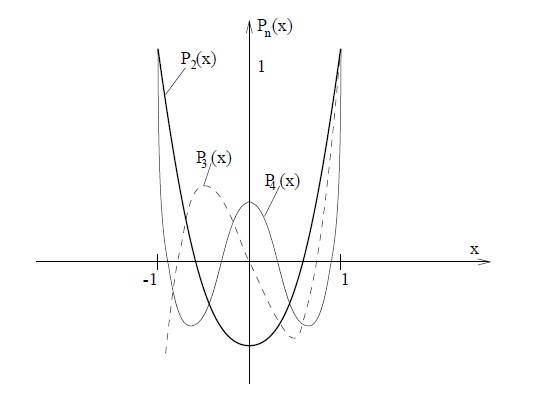
\includegraphics[height=0.82\textheight]{img/5/img2.jpg}
	\end{figure}
\end{frame}
%%%%%%%%%%%%%%%%%%%
\begin{frame}
	\begin{flushright}
    	\textit{Zadanie:} \quad Pokazać, że $P_n(-x) = (-1)^n \cdot P_n(x)$ 
    \end{flushright}
	Wielomiany Legendre'a spełniają równania różniczkowe:
        $$\frac{d}{dx}\bigg[(1-x^2)\frac{dP_n(x)}{dx}\bigg]+n(n+1)P_n(x) = 0$$
        (wynik rozdzielania zmiennych w r. Laplace'a we współrzędnych sferycznych) \newline \par
        \textbf{Ortogonalność: }
        $$\int_{-1}^{1}P_n(x)P_m(x)dx = \left\{\begin{array}{cc}
        0, & m \not= n \\
        \frac{2}{2n+1}, & m = n 
        \end{array}\right.$$
        \begin{flushright}
        	\textit{Zadanie: } \quad Sprawdzić ortogonalność w przypadku dyskretnym.
        \end{flushright}
\end{frame}
%%%%%%%%%%%%%%%%%%%
